\newprob{1719478975}
{
    % active phys p118 *1
    一顆靜止的 Am-241 原子核發生$\alpha$衰變,而成為一顆 Np-237 原子核。
    \par{\par\centering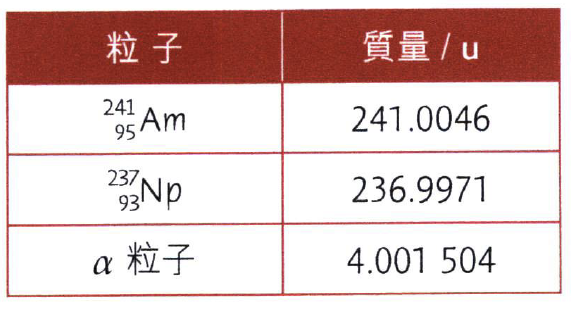
\includegraphics[width=.4\textwidth]{./img/ch3_massenergy_lq_2024-06-27-17-04-09.png}\par}
    \begin{parts}
        \part 衰愛過程中所釋放的能量為多少?\zzh{2}
        \part 假設所有能量皆轉化為動能。
        \begin{subparts}
            \subpart 哪一顆粒子(原子核 Np 還是$\alpha$粒子),分得 更多動能?試詳述之。\zzh{3}
            \subpart 試估計$\alpha$粒子的速率,答案以$c$表示。\zzh{3}
        \end{subparts}
    \end{parts}
}{
    \src{Active Physics p118 *1}
    \par{\par\centering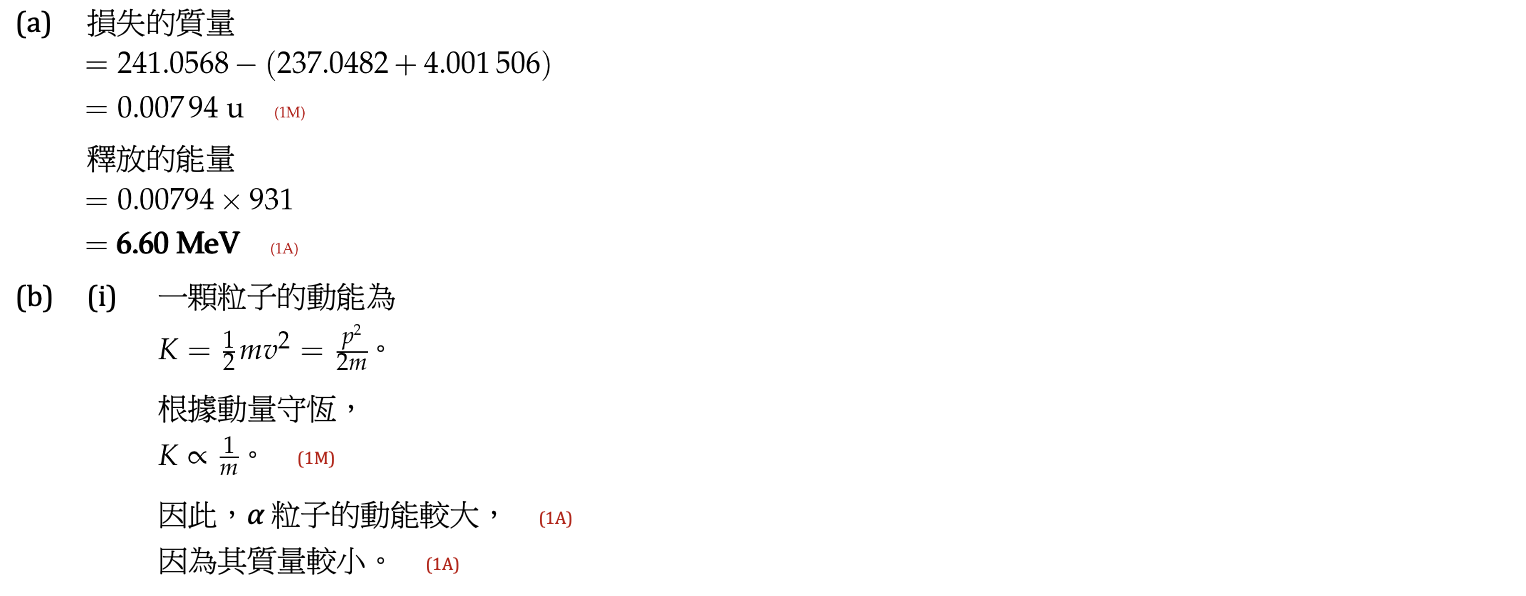
\includegraphics[width=\textwidth]{./img/ch3_massenergy_lq_2024-06-27-17-06-52.png}\par}
}

